\chapter{Metodologia}\label{cap:metodologia}


Este projeto de trabalho de conclusão de curso foi dividido em quatro fases:
Pesquisa, Desenvolvimento, Testes e Monografia.

Durante a pesquisa científica, os artigos referenciados foram explorados com
maior atenção, ao buscar entender os detalhes que implicam
na criação da técnica proposta. Em especial, dois artigos terão maior
atenção inicialmente: \textit{Network Unfolding Map By Vertex-Edge
  Dynamics Modeling}~\cite{VerriNetworkUnfoldingMap2018} e
\textit{Image Segmentation Methods Based on Superpixel Techniques A
  Survey}~\cite{SuperpixelSurvey2020}. O primeiro contém a definição
da técnica LCU, uma dinâmica coletiva sobre redes complexas, o
componente de aprendizagem principal do algoritmo; o segundo será
usado como uma pré-segmentação inicial antes de partir pra construção
da rede complexa. Na Figura~\ref{fig:fluxograma-algoritmo} é demonstrada uma
visão macro do algoritmo.

\begin{figure}[!h]
        \captionsetup{width=8cm}
		\Caption{\label{fig:fluxograma-algoritmo}
          Algoritmo de segmentação semi-supervisionada de imagens}
		\centering
		\UFCfig{}{
			\fbox{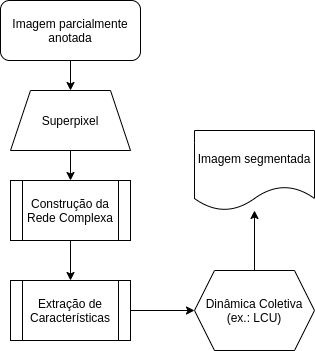
\includegraphics[width=8cm]{figuras/algorithm}}
		}{
			\Fonte{Autoral}
		}
\end{figure}


O desenvolvimento foi concentrado na integração das técnicas
mencionadas acima como uma nova técnica de segmentação de imagens
semi-supervisionada, portanto, estes detalhes são explorados na seção
de resultados sobre as etapas necessárias pra construção e aplicação
do novo algoritmo de segmentação. Por exemplo, a construção da rede
complexa assumirá que cada superpixel será um vértice do grafo com
seus vizinhos baseado na topologia da imagem, a etapa de extração de
características ocorrerá em cada superpixel e a dinâmica coletiva
considerará a anotação parcial da imagem. No fim do algoritmo, os
segmentos da imagem serão subgrafos dessa rede complexa.

Adicionalmente, a implementação do algoritmo nesse trabalho foi
construída de maneira \textit{Open Source} como uma ferramenta de
simulação de segmentação, usando a biblioteca \gls{OpenCV} para que possa
ser testado o algoritmo de segmentação de imagens recebendo pontos
aleatórios de marcação do usuário. Isto simula o caso de um
especialista analisando uma imagem médica, por exemplo.

Na fase de testes, a avaliação dos resultados foi considerado os
principais \textit{datasets} conhecidos para segmentação de imagens,
como o \textit{The Berkeley Segmentation Dataset and Benchmark}
~\cite{MartinFTM01}. É também realizado variações no algoritmo, como
diferentes abordagens para extração de características e variação de
parâmetros na dinâmica coletiva.

Na fase de monografia foram consolidados todos os resultados em um
trabalho acadêmico nas normas da \gls{ABNT}.
